\clearpage
\subsection{Removing redundant features in two-row decisions}
The preceding comparison lowers the row-operation count while leaving the
cost of evaluating row choices visible in the forward stage. The recorded
training data contain 1,923 groups with two source candidates among 2,520
eligible groups. Their algebra supplies an additional way to reduce this cost.

Let $\boldsymbol u$ and $\boldsymbol v$ be two rows with the same leading
integral, and let $u_p$ and $v_p$ be their nonzero leading coefficients.
The two possible elimination updates satisfy
\[
 \boldsymbol v'=\boldsymbol v-\frac{v_p}{u_p}\boldsymbol u,
 \qquad
 \boldsymbol u'=\boldsymbol u-\frac{u_p}{v_p}\boldsymbol v
              =-\frac{u_p}{v_p}\boldsymbol v'.
\]
Their nonzero positions therefore agree. The estimated number of surviving
entries and its square also agree at the finite-field points where both
leading coefficients remain nonzero. For either retained linear score, these
shared terms cancel when we compare the two candidates. The remaining
score difference is
\[
 s(S,1)-s(S,0)=
 \lambda\log\frac{1+n_1}{1+n_0}-\eta,
\]
where $S$ is the current row group, $s(S,i)$ is the score of candidate $i$,
$n_i$ is its number of nonzero entries, and candidate zero is the native
source. The quantity $\lambda$ is the coefficient of source length and $\eta$ is the
coefficient of the native-source indicator. The two retained policies use
$(\lambda,\eta)=(2,0)$ and $(1/2,-0.01)$.

When this comparison selects source zero, the implementation retains that
source without constructing cancellation features. Unsupported modular
expressions already retain the native source, so the same decision also
holds in that case. Other decisions follow the full feature calculation.
The shortcut applies only to the stated sparse linear scores, and detailed
diagnostic traces retain the full calculation.

We compare the shortcut enabled and disabled in 144 complete validation
workflows. All seventy-two pairs agree on source-choice digests, operation
counts, attempt outcomes and exact exports. The enabled path bypasses
cancellation-feature construction in 42,702 row groups. The model-weighted
ratios of decision time, forward-stage time and complete time are
0.345, 0.955 and 0.997, respectively. These ratios compare the same learned policy with and without the shortcut; they describe a reduction in inference cost without changing its algebraic choices.

A separate 4,096-entry cache for modular inverses also preserves all 144 validation reductions. Its forward-stage ratio is 1.002, its decision-time ratio is 1.024, and its complete-time ratio is 0.984. It fails the predefined forward-stage improvement criterion, so the retained implementation leaves this additional cache disabled. The original bounded cache of complete coefficient evaluations remains active.

\subsection{Confirming the reduced inference cost}
We freeze the two-row shortcut after validation and run a second comparison
on the same eight previously reserved profiles. This confirmation preserves
the model weights, seed thresholds, physical inputs, reference bases and
routing rule. It does not supply eight additional independent families.
The smaller native control, deterministic cancellation control, seed model,
row model and combined policy each receive five repetitions on all sixteen
batches, giving 400 workflows.

Every model and control uses the same new executable and temporary-storage
settings. All 400 workflows complete and match their exact reference
coefficients. They use 460 attempts, including sixty failed subset attempts
whose time contributes to the completed workflows. Their selected seed masks, committed operations, row-group
counts and native exports also agree with the corresponding initial trials.
Figure~\ref{fig:integrated-pair-times} separates complete time from the
forward stage in this confirmation~\cite{KiraIntegratedRuntimeData}.

The seed model has a complete-time ratio of 1.155 to the smaller native control, with interval $[1.024,1.316]$. The descriptive interval lies above one. Its forward-stage ratio is 1.083, with interval $[1.001,1.186]$.

The row model has a complete-time ratio of 0.999 to the smaller native control, with interval $[0.992,1.007]$. The descriptive interval includes one. Its forward-stage ratio is 1.041, with interval $[1.017,1.065]$.

The combined policy has a complete-time ratio of 1.159 to the smaller native control, with interval $[1.030,1.319]$. The descriptive interval lies above one. Its forward-stage ratio is 1.097, with interval $[1.010,1.212]$.

For the two-loop sunrise profiles, the seed, row and combined complete-time ratios are 1.397, 0.992 and 1.400. The complete-time intervals are $[1.392,1.402]$, $[0.985,0.998]$ and $[1.388,1.412]$, respectively. The row policy's forward-stage ratio is 1.044, with interval $[1.003,1.085]$.

For the two-loop box profiles, the seed, row and combined complete-time ratios are 0.964, 1.012 and 0.969. The complete-time intervals are $[0.949,0.979]$, $[1.003,1.021]$ and $[0.959,0.979]$, respectively. The row policy's forward-stage ratio is 1.028, with interval $[0.992,1.065]$.

For the three-loop vacuum profiles, the seed, row and combined complete-time ratios are 1.319, 1.003 and 1.317. The complete-time intervals are $[1.129,1.542]$, $[0.996,1.010]$ and $[1.129,1.537]$, respectively. The row policy's forward-stage ratio is 1.041, with interval $[1.007,1.078]$.

For the three-loop ladder profiles, the seed, row and combined complete-time ratios are 1.001, 0.990 and 1.010. The complete-time intervals are $[0.999,1.003]$, $[0.986,0.994]$ and $[1.003,1.017]$, respectively. The row policy's forward-stage ratio is 1.052, with interval $[1.047,1.057]$.

Applying the row policy within the learned-seed workflow gives a complete-time ratio of 1.004 to seed selection alone, with interval $[1.000,1.008]$. Its forward-stage ratio in that comparison is 1.013, with interval $[0.997,1.031]$. These measurements include the model cost and the algebraic consequences of its choices.

The row model's complete-time ratio to the deterministic cancellation rule is 0.993, with interval $[0.983,1.002]$. The deterministic rule receives the same two-row shortcut, which keeps this comparison matched.

The native integration audit verifies that every used seed belongs to the
selected mask and that each learned row attempt loads the frozen policy for
its physical class. It records 404 learned-seed attempts with 147,556 used
selected seeds, and 324 learned-row attempts with 363,759 eligible groups
and 5,795 changes from the native source. These counters show that the
models affect native equation generation and the evolving elimination.

The aggregate row-operation reduction therefore does not establish a reduction
in forward-stage time. The complete-time interval for the row policy includes
one, while always enabling seed selection or both models increases aggregate
complete time. The box cases support a conditional seed-model gain.
The automatic rule remains the rule fixed on validation; the confirmation
results do not retune it.

\begin{figure}[htbp]
\centering
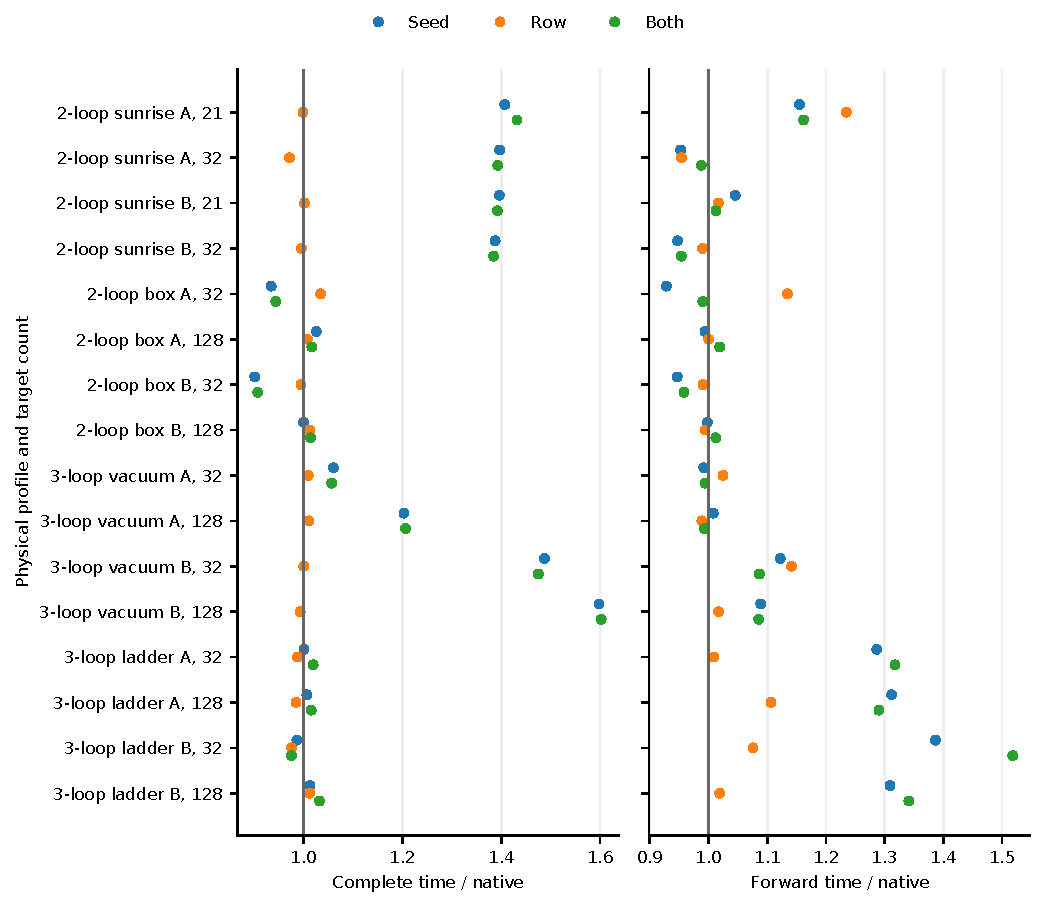
\includegraphics[width=\linewidth]{figures/integrated_pair_times.pdf}
\caption{The implementation confirmation compares the same frozen models with
the smaller native control after reducing two-row inference cost. The left
panel shows complete-time ratios and the right panel shows forward-stage
ratios. Each point uses five repeated complete reductions of the indicated
batch. The physical profiles repeat those in the initial comparison; all
algebraic choices and exact exports remain unchanged.}
\label{fig:integrated-pair-times}
\end{figure}

\clearpage
\subsection{Reducing new targets from a known master basis}
The reference answers above provide an independent benchmark check.
The production interface also accepts only the physical family, target
indices and prescribed master indices. It then determines the target
coefficients through native IBP generation and exact elimination.

To state this distinction mathematically, let $\boldsymbol I$ be the vector
of integrals in the generated system and let $A(d)$ be its IBP coefficient
matrix. The identities give $A(d)\boldsymbol I=0$. Native exact row operations
replace this system by $U(d)A(d)\boldsymbol I=0$, where $U(d)$ represents the
valid elementary row operations. Once elimination expresses all requested
targets through the prescribed masters, it gives
\[
 \boldsymbol I_{\mathcal T}=R_{\mathcal T}(d)\boldsymbol M.
\]
Here $\boldsymbol I_{\mathcal T}$ contains the requested targets,
$\boldsymbol M$ contains the supplied master integrals, and
$R_{\mathcal T}(d)$ is the rational coefficient matrix calculated by Kira.
The learned model chooses seeds and admissible source rows; the exact
identities and row operations determine this relation.

The controller checks that every target has a reduction and that every
integral on its right-hand side belongs to the supplied basis.
An additional integral triggers the fixed seed expansion. The interface
reports incompleteness if the allowed attempts fail. These checks establish
completion relative to the supplied basis under native exact IBP algebra.
They do not establish that an arbitrary supplied basis is globally minimal.
If reference coefficients are available, the interface can additionally
compare them exactly, and its records distinguish these two verification modes.

Eight application checks exercise native, seed, row, combined and automatic
execution on sunrise and box inputs. The reducer receives master indices
without target coefficients. After each run, a separate caller compares the
result with the retained exact reference, and all eight checks pass.
The application record includes input and routing time as well as the complete
reduction time. It excludes lossless evidence compression and optional common
release-integrity checks.

Automatic execution retains the routing rule fixed from validation. It enables
a learned method only in the tested feature classes where validation found
the required advantage, and uses native execution elsewhere. The individual
model modes remain available for controlled comparisons. The reported
model effects concern fixed rational kinematics, a known basis and symbolic
dimension $d$. Generic multiscale reconstruction, unrestricted higher-loop
families and global minimality remain outside this measured domain.
